\documentclass{article}

\usepackage[activate={true,nocompatibility},final,tracking=true,kerning=true,spacing=true,factor=1100,stretch=10,shrink=10]{microtype}
% activate={true,nocompatibility} - activate protrusion and expansion
% final - enable microtype; use "draft" to disable
% tracking=true, kerning=true, spacing=true - activate these techniques
% factor=1100 - add 10% to the protrusion amount (default is 1000)
% stretch=10, shrink=10 - reduce stretchability/shrinkability (default is 20/20)

\usepackage[utf8]{inputenc}
\usepackage{amssymb}
\usepackage{amsmath}
\usepackage{mathtools}
\usepackage{svg}
\usepackage{graphicx}
\usepackage[superscript, biblabel, nomove]{cite}
\usepackage[hidelinks]{hyperref}
\usepackage{cleveref}
\usepackage{tikz}
\usepackage{pgfplots}
\usepackage{datetime}
\usepackage{color}

% Use § for sections
\crefformat{section}{\S#2#1#3}
\crefformat{subsection}{\S#2#1#3}
\crefformat{subsubsection}{\S#2#1#3}

\usepackage{appendix}

% == Remove or comment these out for release
%\usepackage{todonotes}
%\usepackage{draftwatermark}
%\SetWatermarkText{DRAFT}
%\SetWatermarkScale{3}
% ==

\usepackage[utf8]{inputenc}
\usepackage[english]{babel}
\usepackage{amsthm}

% Make itemize bullets slightly smaller
\renewcommand\labelitemi{{\boldmath$\cdot$}}

\newtheorem{theorem}{Theorem}
\theoremstyle{definition}
\newtheorem{definition}{Definition}[section]

\newtheorem{thm}{The`orem}[section] % the main one
\newtheorem{lemma}[thm]{Lemma}

\theoremstyle{plain} % just in case the style had changed
\newcommand{\thistheoremname}{}
\newtheorem{genericthm}[thm]{\thistheoremname}
\newenvironment{namedthm}[1]
  {\renewcommand{\thistheoremname}{#1}%
   \begin{genericthm}}
  {\end{genericthm}}

\begin{document}

% Macros
\newcommand{\HAV}{\textsc{hav}}
\newcommand{\NOM}{\textsc{nom}}


\title{A decentralised payment network and stablecoin\\ v0.7}
\author{Samuel Brooks, Anton Jurisevic, Michael Spain, Kain Warwick}
\date{}

\begin{figure}
    \centering
    %\includesvg[width=0.33\textwidth]{img/block8logo}
    
\includegraphics[width=0.33\textwidth]{img/havvenlogo}
\end{figure}
\maketitle

\hfill

\begin{abstract}
\noindent There is currently no effective decentralised medium of exchange. We propose a decentralised peer-to-peer payment network that does not rely on a central authority to maintain trust and enables a price-stable token for value transfer. Prior to Bitcoin, attempts to create digital currencies were centralised, making them vulnerable to censorship and seizure. Bitcoin’s distributed consensus mechanism protected it from interference, but its fixed monetary policy fostered extreme volatility. Havven solves these problems by issuing a price-stabilised token against a distributed collateral pool which derives its value from the utility of the system. Fees are levied on transactions, and they are dispersed proportionally among collateral holders. Growth in transaction volume thus increases the value of the collateral, which allows the stable token supply to expand to meet demand. The resulting token retains the best features of Bitcoin, while the introduction of price stability enables the payment network to be used for everyday economic purposes.
\end{abstract}	
\vspace{20mm}
\begin{center}
  %\color{gray}
  \small{\textit{\currenttime , \today}}
\end{center}

% \todo[inline]{Incorporate white paper criticisms.}

\pagebreak 

\tableofcontents

% == Remove or comment out this section for release
% \pagebreak
% \section{TODO}
% \listoftodos{}
% ==

\pagebreak

\section{Introduction}

\subsection{Money and Cryptocurrencies}

\noindent The technology of money has three key functions: to act as a unit of account, a medium of
exchange and a store of value. In addition, money should ideally exhibit durability,
portability, divisibility, uniformity, limited supply, and acceptability.
As payment technology has advanced in recent years, it has become increasingly invisible
and it is often lost upon users of money that, like any technology, it can be improved.
Specifically, this means improving the performance of those desirable properties. \\

\noindent Bitcoin is an impressive technological advancement on existing forms of money because it simultaneously improves durability, portability, and divisibility. Further, it does so without requiring centralised control or the enforcement of a nation state from which to derive its value. This fixed monetary policy has protected Bitcoin from debasement and devaluation, allowing it to outperform other forms of money as a store of value. But this has created the potential for short-run volatility as Bitcoin lacks a mechanism to dynamically adjust to changing demand. \\

\noindent Bitcoin has thus tended to be a poor medium of exchange and an even worse unit of account.
In order for something to perform these functions it must remain
relatively stable against the price of goods and services over the short to medium term.

\subsection{Stablecoins}

\noindent A stablecoin is a cryptocurrency designed for price stability, such that it can function both as a medium of exchange and unit of account. It should ideally be as effective for making payments
as fiat currencies like the US Dollar, but still retain the desirable characteristics of Bitcoin, namely
transaction immutability, censorship resistance and decentralisation. \\

\noindent Cryptocurrencies that exhibit these characteristics are clearly a far better form of money; but adoption has been hindered by the volatility inherent in the inflexible monetary policies employed by decentralised systems. Thus stability continues to be one of the most valuable yet elusive characteristics for the technology. Clearly, efforts to create dynamic monetary policies within cryptoeconomic systems is still nascent, and significant research into stable monetary frameworks for cryptocurrencies is required. \\

\noindent The interested reader can also find additional discussion of stablecoins,
cryptoeconomics, competitors, and other related topics on our blog at \href{http://blog.havven.io}{\texttt{http://blog.havven.io}}.

\subsection{Havven}

\noindent Havven is a decentralised stability marketplace, where users requiring stability transact directly with those who provide the collateral to create it. This enables a novel form of representative money in which there is no requirement for a physical asset, thus removing problems of trust and custodianship. The asset used to back the stablecoin is a pool of reserve tokens that collectively represent the system itself; controlling these reserve tokens reflects participation in the Havven system, and they are a proxy for its value. Havven generates fees from users who transact in the stablecoin and distributes them among the holders of the reserve token, compensating them for underpinning the system. Havven therefore rewards those who actively participate in maintaining the stability of the system and charges those who benefit from its utility. These rewards are proportionally applied in response to the active management of the supply of the exchange token such that its price mirrors that of the asset it tracks. \\

\noindent Because we have created a system that generates cash flow for participants, we now have an asset which can be used as the collateral to support the stablecoin with a well-defined market value. The key to this is that the value of the system is measured in US dollars. This allows the system to issue a stablecoin which can be presented and redeemed for a percentage of the collateral tokens valued at \$1. Backing a stablecoin in this way is beneficial because such a cryptoeconomic system does not require trust in a centralised party; each participant has full transparency over how many tokens have been issued against the available collateral at all times. \\

\noindent The two linked tokens and the complex of incentives are described below: \\

\noindent \textbf{Havven}

\vspace{1mm}

\noindent The collateral token, whose supply is static.
The capitalisation of the havvens in the market reflects both the system's aggregate value and the reserve
which backs the stablecoin. Thus, users who hold havvens take on the role of maintaining stability.
Following Bitcoin, the Havven system will appear in upper case and singular; while the havven
token will be lower case and may be plural.

\vspace{2mm}

\noindent \textbf{Nomin}

\vspace{1mm}

\noindent The exchange token - the stablecoin - whose supply floats.
Its price as measured in fiat currency should be relatively stable.
Other than price stability, the system should also encourage some adequate level
of liquidity for nomins to act as a useful medium of exchange. \\

\noindent Each holder of havvens is able to issue a value of nomins in proportion to the dollar value
of the havvens they hold and are willing to place into escrow. If the user wishes to release their escrowed havvens, they must present the system with nomins in order to free their havvens and trade them again.
The holders of this token provide both collateral and liquidity, and in so doing assume some
level of risk. To compensate this risk, such nomin-issuers will be rewarded with fees the system levies
automatically as part of its normal operation. \\

\subsection{Design Rationale}

\noindent This issuance mechanism allows nomins to act as a form of representative money, where each nomin represents a share in the havven value held in reserve. Nomins derive value insofar as they provide a superior medium of exchange, and are effectively redeemable for a constant value of the denominating asset. In this paper, we use US dollars as this asset, but this could be any external and appropriately fungible asset, such as a commodity or a fiat currency. The system incentivises the issuance and destruction of nomins in response to changes in demand, to maintain a constant price. \\

%\noindent The design choice to back the system with a self-referential token was obvious;
%an asset-backed stablecoin with a cryptocurrency basket as reserve will always be inherently
%volatile, despite diversification, and will never be able to achieve the bespoke functionality
%of an asset which derives its value from stability. \\

\noindent In order to issue a nomin, there must be a greater value of havvens escrowed in the system. Overcollateralisation in this way provides confidence that nomins can be redeemed for their face value, even if there is a reduction in the value of the locked havvens. For example, if the collateralisation ratio is set to 100:1 then the price of havvens would need to fall 99\% for the nomin to no longer be overcollateralised. On the other hand, the ratio could be set to 1:1, but any decrease in havven price would mean the currency was no longer overcollateralised. In this situation, it would not be possible for all nomins to be redeemed for their face value, which may cause confidence in the system to drop.  \\

\noindent While overcollateralisation strongly supports a stable nomin price, it simultaneously reduces the efficiency of the system by limiting the utility of the nomin. A ratio of 1:1 provides far greater utility than 100:1, with respect to both the effiicency of the collateral and the revenue generated from transaction fees. There is clearly a trade-off between efficiency and resilience in Havven, which means the collateralisation incentives must therefore not only promote nomin price stability. They must also allow the system to operate as efficiently as possible, whilst maintaining resilience to reduction in the value of the collateral. The design of these incentives is described in detail in section 2. \\

\noindent Due to denominating the value of the stablecoin in an external fiat currency stability is relative only to that currency. In the future the system may support additional flavours of stablecoin that are denominated in other currencies such as the Euro. Denominating the stablecoin in a fiat currency removes the need to respond to macroeconomic conditions, as it benefits from the stabilisation efforts of large institutions acting in fiat markets. \\

\pagebreak

%\section{Design Considerations}

Havven works by providing a set of market incentives that support the stability of nomin value with respect to an external asset.

\todo[inline]{Address how to maintain baseline demand.}
\todo[inline]{Address the role of the Havven foundation.}
\todo[inline]{Outline basic verbs for market players.}

\todo[inline, caption={Functional description refactor.}]{Move analytical subsections from functional description section to the qualitative analysis and/or rationale sections.}
\subsection{Investment incentives}

We consider the reasons why any rational actor would buy havvens. A potential buyer has at least three avenues for making money in Havven:

\paragraph{Capital gains due to the appreciation of havvens:}
Due to its constrained supply, and the intrinsic utility of the stablecoin that it backs, it's reasonable to assume that
havvens will appreciate in price.

\paragraph{Interest accrued from fees:}
If the price of havvens stabilises for long periods of time, fees may be the only source of revenue. Ideally fees are set at a level where they are both high enough to be an incentive for rent-seekers to hold havvens in the long term (thus assuming the risk of providing collateral for the system) and low enough not to be a disincentive for ordinary users to transact in nomins.
It is desirable, perhaps in a future world dominated by micropayments, for these fees to be negligible for end users, while still being macroeconomically important for the system, and for those who capitalise it.

\paragraph{Arbitrage profit:}
It is the arbitrageurs who will ultimately bring the price of nomins back into balance by a triangular circuit through nomins, havvens, and the external (crypto or fiat) markets. Arbitrageurs might hold havvens for a short time in order to pursue this strategy.


\pagebreak
\subsection{Fees}

There are several key considerations with respect to fee design:

\subsubsection{Fee design considerations}

\paragraph{The purpose of fees}

Fees are intended to be redistributed to actors who support the stability of the system. A fee pool will be distributed periodically for this purpose.
If the system determines that the nomin price is too low, then fees could be burned. If the price is too high then the system could sell these back
into the system at a discounted rate. The fee collection rate will also be a direct measure of the velocity of money in Havven. It's in the interest
of havven holders to maximise liquidity in order to maximise their return.

\paragraph{Fee beneficiaries}

One possibility would be simply to award fees to any holder of havvens,
but in this situation holders can get all the benefit without taking any risk.
Although in the aggregate, it would be better for havven-holders if everyone issued nomins,
the marginal return for any single player (who cannot issue a large fraction of all circulating nomins)
of actually issuing them would not outweigh the risk they take on in doing so. If a user can issue 1\% of circulating
nomins, then doing so will only increase their fee takings by 1\%. Hence rational actors would not be incentivised to issue nomins at all.
This is a classic tragedy of the commons.

\noindent In order to avoid this situation, we must improve the marginal benefit of issuing nomins into circulation.
Hence, fees must be paid to those who \textit{issue} nomins, not just those who hold havvens.

\paragraph{Fee collection}

The system can charge fees whenever any value is transferred, or any state is updated.
\noindent Different fee rates have different macroeconomic effects. We might in general like to set higher havven than nomin transfer fees, making the stablecoin itself a lower friction market in order to incentivise its use for exchange. Meanwhile, issuance and redemption fees will change the difficulty of entering and exiting the issuance game. \\

\noindent It is also possible for fees to float. The fee schedule could be altered dynamically in order to stabilise the system. It is even conceivable that the system could set negative fee rates if it needed to and charge punitive fees if a user is above the targeted utilisation ratio. For example, if nomin liquidity is low, meaning the system wants to incentivise issuance, then nomin transfer fees could increase, thus having the combined effect of increasing the interest accrued by issuers (thus incentivising issuance) and at the same time making it more expensive to transact in nomins. This would reduce demand and decrease the liquidity requirements. \\

\noindent Of note, fees are antithetical to arbitrage. The higher the fee, the higher the transaction friction, and the harder it is to make money by arbitrage. For example, if exchange fees amount to 1\% per trade, then a full arbitrage cycle between all three markets, (nomins, havvens, and fiat) will cost in excess of 3\%. So it would not make sense to undertake arbitrage until such a time as the quoted exchange rate is misvalued by more than 3\% relative to the cross exchange rate. Hence, fees compete with arbitrage to stabilise price. Lower fees allow tighter stabilisation, within a window exactly in proportion with the fee rates themselves.

\subsection{Encouraging liquidity}

\noindent It's desirable that when actors issue nomins they are actually injected into the liquidity pool for their intended use,
rather than being held by the same actor in order to benefit from both the receipt of fees while retaining the option of using those nomins to rapidly release their havvens.
In this manner they would accrue fees, but take on none of the risk of spending those nomins, for they always have an instantaneous option to liquidate their position and escape.
On the other hand, an actor who had done the economically-desirable thing and issued nomins to the market would be forced to buy them back before redeeming their escrowed havvens.

\subsubsection{Non-discretionary Issuance}

One possibility is to simply provide an issuer no control over the tokens they issue. That is, when a quantity of nomins is issued, they are generated by the system, which then places a sell order at the current going rate for that quantity on an exchange on the behalf of the issuer. When the order is filled, the proceeds in ether are remitted to the issuer. \\

\noindent Conversely, when a quantity of nomins is burned, they must first be obtained from the open market. In this way, a user would indicate an intention to burn, providing sufficient value to buy the proposed quantity of nomins, and the system would bid for that quantity on their behalf, thereby liquidating the user's havven position once the nomins have been obtained. \\

\noindent So one might consider there to be a formal distinction between wallets that issue tokens and those that do not. In this vein, one might envisage an extra fee to be charged to directly transfer nomins (rather than buying from the market) into a wallet that has an outstanding quantity of nomins it has previously issued, but not burnt. The result of this is that it would be less reasonable for an agent to sit on nomins in order to burn them in future as it is more advantageous in times of relative stability to simply buy them from the market. \\

\pagebreak 

\subsection{Price discovery}

One of the key challenges with denominating a cryptocurrency in a fiat currency is the
fundamental link this creates to the centralised world. When the denominating currency exists
external to the blockchain ecosystem, some bridge must be built so that the system can act with
knowledge of external information.
We recognise that a decentralised price-finding mechanism would be our preferred approach.
Research into this mechanism is on our horizon, and future versions of this white paper will contain
our results.
However, in order to reclaim system performance, we can trade some of the trustlessness of the design, for example by
a trusted ``Oracle'' service, which transmits knowledge of the external world into the system, building a causal link.


\subsection{Utilisation Ratio} Even though rational actor modelling suggests that the price of nomins and havvens will equilibrilate
given that an agent may pay up to some multiple of the market value of a nomin in order to release escrowed havvens, we are aware that there may be some
prevailing macroeconomic or psychological influences relating to an undercollateralised position
(i.e. if the value of the collateral pool is less than the issued stablecoin). As such, our modelling incorporates the notion of a ``utilisation ratio''
\(0 < U < 1\), such that the system is over-collateralised in an attempt to counteract these potential issues. It may be that resolving an
optimised utilisation ratio is beyond the ability of our agent-based modelling to determine, and as such, selecting this may need to be
informed by the activity of a live system. Thus it is currently intended for Havven to initially include in its governance model the power
to correct the utilisation ratio. This power can be removed over time as the system is proven, perhaps directly linked to some parametric milestones such as nomin velocity and stability.

%\paragraph{Direct Redemption} Direct redemption is a system design option to allow a holder of nomins to redeem any escrowed havvens. This option allows more efficient redemption of nomins for the backing value, however introduces the difficulty of liquidating another actor's escrowed havvens and interrupting their collection of fees. This can be solved by adding a premium to the price of an escrowed havven (potentially user-defined) over the current value. This premium would need to be paid in ether as to preserve the symmetric issuance and destruction of nomins. \\

\pagebreak

\section{System Description} Havven is a dual-token system that, combined with a set of novel incentive mechanisms, stabilises the price of the nomin with respect to an external asset. Users of the nomin token pay the owners of the havven token for collateralising and stabilising the system. \\

\noindent The havven token incentivises those who hold it to serve two functions:

\begin{itemize}
\item{To provide the system with collateral.}
\item{To participate in the stabilisation of the nomin price.}
\end{itemize}

\paragraph{Collateralisation}

\noindent Confidence in stability of the nomin begins with overcollateralisation, so that the value of escrowed havvens is greater than the value of nomins in circulation. The value of havvens is derived internally by the system as a function of the demand for nomins; this decouples the value of the collateral pool from market speculation. \\

\noindent As long as the ratio of total nomin value to total havven value remains favourable, there is sufficient backing in the underlying collateral pool to ensure that nomins can be redeemed for their face value. The redeemability of a nomin for the havvens against which it was issued strongly supports a stable price.  

\paragraph{Incentives}

\noindent Havven rewards those that have issued nomins. These rewards are derived from transaction fees and are distributed in proportion with how well each issuer maintains the correct nomin supply. The system monitors the nomin price, and responds by adjusting its targeted global supply, which individual issuers are incentivised to move towards. \\

\noindent Where volatility persists, stronger stabilisation mechanisms may be applied such as automated collateral recovery. Where a significant portion of nomins are being used for hedging, (and hence not generating transaction fees) a charge can be applied to ensure that the cost of utility for hedging is not being solely borne by transactions.

\newpage

\subsection{Definitions}

\noindent We first introduce the core system variables:

\begin{align*}
H &:= \text{havven quantity} & N &:= \text{nomin quantity} \\
P_h &:= \text{havven price}  & P_n &:= \text{nomin price} \\
\end{align*}

% \todo[inline]{Consider renaming havven price symbol to reflect that it is computed from income}

\noindent All havven tokens are created in the initial system state, so $H$ is constant. The quantity of nomins, $N$, floats in response to the actions of havven holders.The Havven system needs to incentivise havven holders to maintain $N$ such that the nomin price, $P_n$, is stable at \$1.\\

\noindent In Havven, the collateralisation ratio measures the value of nomins against the value of havvens:

\begin{equation}
C = \frac{P_n * N}{P_h * H} \label{eq:collateralisation}
\end{equation}

\noindent We will subscript variables with $t$ to indicate the value of that
variable at a given time.

\pagebreak

\subsection{Nomin Equilibrium Price} The law of supply and demand states that there exists some supply of nomins, $N_{opt}$, where the related level of demand yields an equilibrium price of \$1. This quantity is associated with an optimal collaterisation ratio, $C_{opt}$. We visualise this equilibrium below with a hypothetical demand curve, D, and a supply curve, S.  \\

% \todo[inline]{curved lines}
% \todo[inline]{make diagrams pretty}
\begin{center}
\begin{tikzpicture}[scale=3]

% draw axes
\draw [<->, thick] (0,2) node (yaxis) [above] {$P_n$} |- (2.5,0) node (xaxis) [right] {$N$};

% draw intersecting lines
\draw (0.5, 0.5) coordinate (a_1) -- (2,1.8) coordinate (a_2) node[pos=0.0, left] {S};
\draw (0.5, 1.8) coordinate (b_1) -- (2,0.5) coordinate (b_2) node[pos=1.0, right] {D};

% calculate coordinate of intersection
\coordinate (c) at (intersection of a_1--a_2 and b_1--b_2);

\draw[dashed] (yaxis |- c) node [left] {$1$} -| (xaxis -| c) node[below] {$N_{opt} = \frac{C_{opt} * P_h * H}{P_n}$};

\end{tikzpicture}
\end{center}

\noindent The system is unable to influence the demand for nomins. We assume that some level of demand exists given the utility of nomins as a stable cryptocurrency. Although demand cannot be manipulated, the supply of nomins is controlled by havven holders, whose issuance incentives are in turn controlled by the system. It follows that as we require a fixed price $P_n = \$1 $ and are unable to control either $P_h$ or $H$, we must manipulate $C_{opt}$ such that $N = N_{opt}$ in order to satisfy our requirement.

\subsection{Intrinsic Havven Value}

\noindent Being a freely-tradable ERC20 token, havvens will have a market price.
However, using this for $P_h$ would expose the collateralisation ratio computation
to speculative price shocks. Instead, the ``true'' price of a havven is computed as a
function of the transaction fees that the system charges. In this way we connect the
computed price of the havven directly with demand for nomins.
Price increases will allow an expansion in the money supply exactly when demand has increased. \\

\noindent We define the value of a havven as a share in the discounted sum over past fee returns.
In this way the price is not vulnerable to instantaneous volume spikes, while
taking the most recent transaction volumes to be the most highly-correlated with future volumes.

\begin{equation}
    P_{h,t} = \frac{1}{H} \sum_{t'=1}^{t} \frac{F_{t - t'}}{(1 + r)^{t'}} \label{eq:price}
\end{equation}

where

\begin{align*} 
& P_{h,t} \text{ is the price of one havven at time } t  \\
& F_t \text{ is the total fees collected in period } t\\
& H \text{ is the total supply of havvens}  \\
& r \text{ is a falloff term}  \\
\end{align*}

\noindent This can be computed efficiently, because $P_{h,t+1} = \frac{P_{h,t} + F_t}{r}$. 
Further, if it is assumed that the average fee take is approximated by $F_t$, and $t$ is large, then

\begin{equation}
    P_{h,t} \approx \frac{1}{H} \sum_{t'=1}^{\infty} \frac{F_t}{(1 + r)^{t'}} = \frac{F_t}{H \cdot r}
\end{equation}

\newpage

\subsection{Issuance and Collateralisation} 

% \todo[inline]{separate wallets from accounts}

\noindent Havven's goal is to remain overcollateralised. In order to do so, the system defines a collaterisation target:

\begin{equation}
0 < C_{opt} < 1  \label{eq:target}
\end{equation}

\noindent It is necessary at this point to distinguish between the nomins in a wallet $N_i$ (equity) and the nomins that have been issued by that wallet $\check{N_i}$ (debt). Note that globally, the $\sum_{i}N_i = \sum_{i}\check{N_i}$, as all circulating nomins were issued by some wallet. However, a given wallet may have a balance different from its issuance debt.\\
% \todo[inline]{Make sure this equity/debt language is not too security-like.}

\noindent Hence we can define the collateralisation ratio for an individual wallet $i$ in terms of its issuance debt:

\begin{equation}
C_i = \frac{P_n \cdot \check{N_i}}{P_h \cdot H_i}  \label{eq:individualcollat}
\end{equation}

\noindent The system provides incentives for individual issuers to bring their $C_i$ closer to $C_{opt}$ while maintaining $C_{opt}$ itself at a level that stabilises the price.

\paragraph{Nomin Issuance}

\noindent The nomin issuance mechanism allows Havven to reach its collaterisation target. Issuing nomins escrows some quantity of havvens, which cannot be moved until they are unescrowed. The quantity of havvens $\check{H_i}$ locked in generating $\check{N_i}$ nomins is:

\begin{equation}
\check{H_i} = \frac{P_n \cdot \check{N_i}}{P_h \cdot C_{max}}  \label{eq:escrowed}
\end{equation}

\noindent Under equilibrium conditions, there is some $\check{H_i} \leq H_i$ when $C_i = C_{opt}$, which the issuer is incentivised to target. These incentives are provided in the form of transaction fees, discussed in section 2.4. It is important to note that the issuer may voluntarily increase their $C_i$ up to the limit of $C_{max}$; for example if they anticipate a positive movement in $C_{opt}$. $C_i$ may never exceed $C_{max}$, except by price fluctuations, and in such circumstances, issuers are rewarded for bringing $C_i$ back under $C_{max}$. \\

\noindent After generating the nomins, the system places a \textbf{limit sell} order with a price of \$1 on a decentralised exchange. This means that the nomins will be sold at the current market price, down to a minimum price of \$1 USD. If we assume implementation on Ethereum, then the nomins are sold for ETH, with the proceeds of the sale remitted to the issuer.

\paragraph{Nomin Destruction}

\noindent In order to access the original havvens that have been escrowed, the issuer must return the same quantity of nomins to the system to be burned. This is a main way 
an issuer can reduce their collateralisation ratio. If an issuer does not possess the required nomins, they can be purchased on the open market.

\subsubsection{Issuance Example}
% \todo[inline]{Finish the example. I don't really know if dealing with nomin price changes here is right, before introducing fees.}

\begin{enumerate}
\item{Bob purchases 100 havvens at \$1 each, total value \$100. The maximum collateralisation ratio $C_{max}$ is 0.5, the optimum collateralisation ratio $C_{opt}$ is 0.4 and the nomin price $P_n$ is \$1.}
\item{Bob decides to issue nomins up to $C_{opt}$. By equation \eqref{eq:escrowed}, the system generates 40 nomins and escrows 80 of his havvens, locking \$80 worth of value in the system $ (\check{N_i} \cdot C_{max})$.}
\item{The system sells the nomins on the market for \$40 worth of ether, transferring it to his wallet}.
\item{The havven price drops to \$0.90. The value of his havvens has decreased to \$90 which means his $C_i$ has increased to 0.44, greater than $C_{opt}$. The system escrows more of Bob's havvens to maintain the value of the locked collateral.}
\item{By \eqref{eq:escrowed} the system escrows an extra 8.9 of his havvens. He now has 88.9 havvens escrowed. The value locked in the system remains unchanged at \$80.}
\item{The havven price then increases back to \$1. The value of his havvens has increased to \$100 and his $C_i$ has decreased back to 0.4. The system releases the 8.9 havvens back to Bob and he has 80 escrowed.}
\end{enumerate}

\noindent The above example has illustrated how the system maintains the value of the underlying collateral by adjusting the quantity of a user's escrowed havvens as the havven price changes.

%\subsubsection{Price changes (Table here maybe?)}

%\noindent \emph{What happens if the price of havvens changes?} \\

%\noindent All issuance of nomins is done at the current $P_h$. However, when $P_h$ changes, the quantity of escrowed havvens changes with it (not the \emph{value}). An increase in $P_h$ means that fewer of Bob's havvens are escrowed. In contrast, a decrease in the $P_h$ means that more of his havvens are escrowed. This process occurs automatically in order to ensure that the system remains overcollateralised. \\ 

%\noindent \emph{What happens if the price of nomins changes?} \\ 

%\noindent In order to release escrowed havvens, Bob must return the same quantity of nomins that he issued. This means that if $P_n$ has increased in the market, he will need to spend more ether than he received when he issued in order to release his havvens. Conversely, if $P_n$ has decreased, Bob will need to spend less in order to release his havvens.

%\subsubsection{Global collaterilisation Ratio}

%\noindent Havven can ensure that nomins are overcollateralised at the time of issuance, however, a reduction in $P_h$ lowers the value of the escrowed havvens. The global collaterilisation ratio is defined as the total value of nomins divided by the total value of havvens:

%$$ U = \frac{P_n * N}{P_h * H}.$$ \\

%\noindent Intuitively, if $U = 1$, the value of nomins and havvens are equal. Hence, given our overcollateralisation property, the system targets $U <  1$. To do this, Havven only allows the issuance of nomins up to a maximum collaterilisation ratio.

%\subsubsection{Unique Collateralisation Ratio}

% \noindent Given the need to adjust the supply of nomins, an optimum collaterilisation ratio is defined as the point at which maximum incentives are applied:

% $$ 0 \leq U_{opt} \leq U_{max} \leq 1.$$

% \noindent Each havven holder that has issued nomins has a unique collaterilisation ratio, $ U_i $. The system can measure the degree to which their $ U_i $ is above or below the optimum and reward them accordingly. In this way the system incentivises the issuance and destruction of nomins. $ U_{opt} $ is defined formally below in terms of $ P_n $. As  the nomin price diverges from the desired \$1, the incentive to either expand or contract nomin supply increases.

\newpage
\subsection{Transaction Fees} Havven needs a direct incentive mechanism that can correct changes in the global collaterisation ratio, $C$, when the price of havvens or nomins changes. \\

\noindent Some of the equations below are defined in the discrete time domain and are referenced with a subscript $t$. These will be specifically used in our game theoretic modelling.

\subsubsection{Nomin Transaction Fees} Every time a nomin transaction occurs, the Havven system charges a small transaction fee. Transaction fees allow the system to generate revenue, which it can distribute to havven holders as an incentive to maintain nomin supply at $C_{opt}$. \\

\noindent The fee rate charged on nomin transactions is $\alpha_c$. It is constant and will be sufficiently small that it provides little to no friction for the user.\\

\begin{equation}
\alpha_c = k \ \label{eq:5}
\end{equation}

\begin{center}
\begin{tikzpicture}[scale=3]

% draw axes
\draw [<->, thick] (0,2) node (yaxis) [above] {$\alpha_c$} |- (2.5,0) node (xaxis) [right] {$P_N$};

% draw one line
\draw (0.0, 0.75) coordinate (a_1) -- (2.4,0.75) coordinate (a_2);

\coordinate (c) at (1.75, 0.75);

\draw[dashed] (yaxis |- c) node [left] {k};

\end{tikzpicture}
\end{center}

\noindent We may then express the total fees collected in period $t$, $F_t$, as a function
of the velocity of nomins $v_t$ and the total nomin supply $N_t$:

\begin{equation}
    F_t = v_t \cdot \alpha_c \cdot N_t
\end{equation}

\newpage
\subsubsection{Fees Received by Havven Holders}

\noindent The fee rate paid to a havven holder that has escrowed is $\alpha_r$.
The actual fee they receive is $\check{H_i} \cdot \alpha_r$, being proportional with the value they stake.
The received fee rate changes with respect their unique collaterilisation ratio, $C_i$.
It increases linearly to a maximum $\alpha_{base}$ at the optimal collaterilisation ratio $C_{opt}$, before quickly
diminishing as $C_i$ approaches the maximum collaterisation ratio $C_{max}$. 

\noindent This function is designed to encourage havven holders to constantly
target the optimal collateralisation ratio, by rewarding them with greater
fees if they do so.\\


 % \todo[inline]{figure out whether t stays}

\begin{equation}
\alpha_{r,t,i} = \alpha_{base,t} \cdot \mathcal{F}_{i,t}(C_{i,t}, C_{opt}, C_{max,t})  \label{eq:feesreceived}
\end{equation}

\begin{equation}
\mathcal{F}_{i,t}(C_{i,t}, C_{opt,t}, C_{max,t}) = 
\begin{cases}
 \frac{C_{i,t}}{C_{opt,t}} &\mbox{when } C_{i,t} \leq C_{opt,t} \\[1em]
 \frac{C_{max,t} - C_{i,t}}{C_{max,t} - C_{opt,t}} &\mbox{when } C_{opt,t} \leq C_{i,t} \leq C_{max,t} \\[1em]
 0 &\mbox{otherwise}
 \end{cases}
 \label{eq:7}
\end{equation}

\begin{center}
\begin{tikzpicture}[scale=3]

% draw axes
\draw [<->, thick] (0,2) node (yaxis) [above] {$\alpha_r$} |- (2.5,0) node (xaxis) [right] {$C_i$};

% draw two lines
\draw (0.0, 0.0) coordinate (a_1) -- (1.75,0.75) coordinate (a_2);
\draw (1.75, 0.75) coordinate (a_1) -- (2.25,0.0) coordinate (a_2);

\coordinate (c) at (1.75, 0.75);
\coordinate (d) at (2.25, 0.0);
\coordinate (e) at (0.00, 0.00);

\draw[dashed] (yaxis |- c) node [left] {$\alpha_{base}$} -| (xaxis -| c) node[below] {$C_{opt}$};
\draw[dashed] (yaxis |- e) node [left] {$\alpha_{base}$} -| (xaxis -| d) node[below] {$C_{max}$};

\end{tikzpicture}
\end{center}

\noindent This fee distribution curve encourages havven holders who have escrowed to maintain their $C_i$ at $C_{opt}$.  \\

\newpage

\subsubsection{Base Fee Rate}

Let us define the total fees paid to havven holders $F_{r,t}$: \\

\begin{equation}
F_{r,t} = \sum_{i} \check{H_i} \cdot \alpha_{r,t,i} \label{eq:totalfeesreceived}
\end{equation} \\

\noindent Havven requires that the total fees collected from users has to be equal to the total amount of
fees paid to the havven holders, so that $F_{r,t} = F_t$. Substituting our earlier definition \eqref{eq:feesreceived} for $\alpha_{r,t,i}$ and solving for $\alpha_{base,t} $: \\

\begin{equation}
\alpha_{base,t} = \frac{F_t}{\sum_{i} \check{H_i} \cdot \mathcal{F}_{i,t}(C_{i,t}, C_{opt,t}, C_{max,t})} \label{eq:10}
\end{equation} \\

\noindent We have now defined the maximum fee rate, $\alpha_{base}$, in terms of the fees collected, $F_t$. This rate should be achieved when an individual's $C_i$ is at $C_{opt}$. \\

\noindent The definition of $C_{opt}$ must therefore provide the following incentive. If $P_n > 1$ then the system must encourage more nomins to be issued. If $P_n < 1$, the system must encourage nomins to be burned. 

\newpage

\subsection{Collateralisation Ratio}
\subsubsection{Optimal Collateralisation Ratio}

\noindent The optimal collaterilisation ratio $C_{opt}$ is a target for havven holders to reach in order to maximise the amount of fees they receive. $C_{opt}$ is defined in terms of $P_n$ such that havven holders can influence the price of nomin through directly controlling the supply of nomin (a havven holder can change their individual collaterilisation ratio by buying or issuing more nomins). \\
 
\noindent The function for $C_{opt}$ given below provides our dynamic target for havven holders based on the price of nomin. The curve shows that the when $P_n$ is close to \$1, $ f'(P_n) $ is small. However, the further $P_n$ diverges from \$1, the larger the derivative becomes, providing an increasing incentive (via fees) for a havven holder to move toward $C_{opt}$.

\begin{gather} 
\begin{align}
\begin{split}
C_{opt,t} &= f(P_{n,t}) * C_t  \\ 
f(P_{N,t}) &= max(\sigma * (P_{N,t} - 1)^{\phi} + 1, 0) \\
& 0 \leq \sigma, \text{ the price sensitivity parameter} \\
& \phi \geq 1, \text{ the flattening parameter} \\
\end{split}
\end{align}
\end{gather}


\begin{center}
\begin{tikzpicture}[scale=1.15]
\begin{axis}[
    axis lines = left,
    xlabel = $P_N$,
    ylabel = {$f(P_N)$},
    xtick = {1},
    ytick = {0},
    y label style={at={(axis description cs:.15,1.00)}, rotate=270,anchor=south},
    x label style={at={(axis description cs:1.05,.13)},anchor=north},
]
\addplot[
domain=0:2,
range=0:2
]
{(x-1)^3 + 1};
\addplot [
domain=0:2,
range=0:2,
dashed
]  
 {x};
 \addplot[dashed, samples=50, smooth,domain=0:6] coordinates {(1,1)(1,0)};
\end{axis}
\end{tikzpicture}
\end{center}

\newpage

\subsubsection{Maximum Collateralisation Ratio}

\noindent Havven seeks to maintain $C \leq C_{opt} < C_{max} < 1$, in order to remain sufficiently overcollateralised. It might seem intuitive that $C_{max}$ should be a static value. However, since $C_{opt}$ changes linearly with $P_n$ and inversely with $P_h$, there are several situations where $C_{max}$ may need to change. Below we define $C_{max}$. \\

\begin{equation}
\label{eq:12}
C_{max,t} = 
\begin{cases}
 C_{base,t} &\mbox{when } C_{opt,t} \leq C_{base,t} \\[1em]
 a * C_{opt,t} &\mbox{otherwise}.
 \end{cases}
\end{equation}

\begin{center}
\begin{tikzpicture}[scale=3]

% draw axes
\draw [<->, thick] (0,2) node (yaxis) [above] {$C_{max}$} |- (2.5,0) node (xaxis) [right] {$C_{opt}$};

% draw intersecting lines
\draw (0.0, 0.75) coordinate (a_1) -- (0.75,0.75) coordinate (a_2);
\draw (0.75, 0.75) coordinate (a_1) -- (1.8,1.8) coordinate (a_2);

% calculate coordinate of intersection
\coordinate (c) at (0.75,0.75);

\draw[dashed] (yaxis |- c) node [left] {$C_{base}$} -| (xaxis -| c) node[below] {$C_{base}$};

\end{tikzpicture}
\end{center}

\newpage
\section{System Analysis}

\subsection{Nomin Demand and Havven Value}

\noindent Being freely-tradable tokens, havvens will have a market
price which, like the nomin price, can be measured with an oracle. Initially,
while nomin demand is low, a seven day rolling average of the market price
will be used for both havvens and nomins. This rolling average is designed to
smooth out fluctuations in the market price and increase the cost of
attacking the system.\\

\noindent However, once nomin transaction volume is sufficiently high, we may
instead estimate the value of a havven by the fees it is likely to accrue.
This value, which implicitly measures nomin volume, would allow issuance
incentives to directly reflect changes in nomin demand. By using this
value instead of the havven market price, the system can avoid the
influence of speculation, since the permitted nomin supply would expand
and contract in line with actual usage. \\

\noindent While the system cannot perfectly determine future fee returns and
hence nomin demand, it is possible to estimate as a function of the
transaction fees that the system has recently generated. This computation is
designed not to be vulnerable to instantaneous volume spikes, while taking
the most recent transaction volumes to be the most highly-correlated with
future volumes:
\vspace{3mm}

\begin{equation}
    V_{t} \ = \ \sum_{t'=1}^{t} \frac{F_{t - t'} \cdot P_{n,t - t'}}{{(1 + r)}^{t'}} \label{eq:price}
\end{equation}

with
\begin{align*} 
V_{t} \ \ & \text{ the system's valuation of a havven at period } t  \\
F_t \ \ & \text{ the total fees collected in period } t\\
P_{n,t} \ \ & \text{ the nomin price at period } t\\
r \ \ & \text{ a falloff term}  \\
\end{align*}

\noindent This can be computed efficiently, because \(V_{t+1} = \frac{V_t \ + \ F_t \cdot P_{n,t}}{1 + r}\). 
Further, for large enough \(t\), if it is assumed that \(P_n \approx \$1\) and that current fees are close to
future ones, so that \(F_t \approx F_{t'}, \ t < t'\), then:

\vspace{2mm}

\begin{equation} 
    V_t \ \approx \ \sum_{t'=1}^{\infty} \frac{F_t}{{(1 + r)}^{t'}} \ = \ \frac{F_t}{H \cdot r} \label{eq:havvenvalue}
\end{equation}

\vspace{3mm}

\noindent Consequently, \(\frac{1}{r}\) approximates the number of periods for
a havven to yield a fee return of \(V_t\). A judicious choice of \(r\) can then
yield a \(V_t\) which underestimates the market price of havvens (which also
incorporates, for example, capital gains), while not unduly constraining
nomin supply.

\newpage

\subsection{Fee Evasion}

\noindent Being implemented with smart contracts, Havven is potentially
vulnerable to its tokens being wrapped by another smart contract which takes
deposits, and replicates all exchange functionality on redeemable IOU tokens
it issues. These wrapped tokens could then be exchanged without incurring fees.
We consider this situation unlikely for a number of reasons. \\

\noindent First, the fees are designed to be low enough that most users
shouldn't notice them, so they will not in general be strongly motivated to
switch to a marginal and less trustworthy alternative. Additionally, transfer
fees will still be charged upon deposit into and withdrawal from
token-wrapping contracts, which partly constrains the utility of the wrapper.

\noindent Second, network effects are tremendously important for currencies;
in order to have utility a token must be accepted for exchange in the
marketplace. This is challenging enough in itself, but a wrapped token must
do this to the extent that it displaces its own perfect substitute: the token
it wraps.
In Havven's case, this would undermine its built-in
stabilisation mechanisms, which become more powerful with increased
transaction volume. Consequently, as a wrapped nomin parasitises more of the
nomin market, it destroys the basis of its own utility, which is that nomins
themselves are stable.

\noindent Finally, it is unlikely that a token wrapper will be credible, not
having been publicly and expensively audited, while its primary function
undermines the trustworthiness of its authors. \\

\noindent Even as token wrapping may appear unlikely to the authors, there
are at least two remedies which can be instituted to resolve this. \\

\noindent It would be a simple matter to implement a democratic remedy,
weighted by havven balance, by which havven holders can freeze or confiscate the
balance of any contract that wraps assets. Those havven holders are
incentivised not to abuse this system for the same reason that bitcoin
mining pools do not form cartels to double-spend: because abuse of this
power would undermine the value of the system, and thus devalue their
own holdings.

\noindent The credible threat of such a system existing is enough to
discourage token wrappers from being used, even if they are written, since
any user who does so risks losing their entire wrapped balance.

\noindent An alternative solution is to institute a hedging fee, charged on static nomin
balances. Such a fee could be discounted against transfer fees so that it
encourages general token velocity, and imposes a cost on those who buy nomins
simply in order to hedge, and are thus a risk for the network. Under this
model, a token wrapper would not dodge this fee: the full balance that was
wrapped will not be available at the time of unwrapping.

\newpage

\subsection{Issuance Case Study}

\noindent In this section we illustrate how Havven's incentives encourage havven holders to
maintain stability.

\noindent In \ref{subsubsec:practicalissuance}, we first present a simplified example the practical issuance
dynamics for a havven holder, Bob, if he targets \(C_{opt}\). In the second part, \ref{subsubsec:coptimality},
we examine the optimality of following this strategy with a more sophisticated model
of the mechanism as a two-player game. \\

\noindent It should be noted that these are simply illustrative examples to give the 
reader a feel for the nature of the system's issuance dynamics. This
section is partly an adaptation of the calibrated analysis results presented
in much greater depth in as part of the economic analysis of Havven performed by
\href{http://cryptecon.org/}{\textcolor{blue}{cryptecon}}, which can be found in
its entirety \href{https://havven.io/uploads/havven_cryptecon_report_may_2018.pdf}{\textcolor{blue}{here}}. \\

\noindent The cryptecon investigation concluded that the Havven system
generally stabilises the nomin price at \$1, but most of the supporting
apparatus has been omitted in this white paper. Therefore, an interested reader should
consult that reference for further details and an explanation of the assumptions
which underly its results. \\

\noindent Throughout this section we will assume implementation upon Ethereuem, therefore
in this example, the system will buy and sell nomins in exchange for ether, but this could be 
substituted with any asset tradeable in a decentralised way. \\

\newpage
\subsubsection{Practical Issuance Dynamics}
\label{subsubsec:practicalissuance}

\noindent \textbf{Initial Conditions} \\

\noindent Bob decides to purchase 100 havvens at \$1 each.
The system is in price equilibrium, with the global collateralisation
ratio \(C\) equal to the optimal collateralisation ratio
\(C_{opt}\). We will denote Bob's personal \(H\) and \(C_i\) with
\(H_{bob}\) and \(C_{bob}\). The initial conditions are then as follows:

\begin{align*}
    C_{max} &= 0.5 & C_{opt} &= 0.4 & C &= 0.4 \\
    P_n &= 1 & P_h &= 1 & H_{bob} &= 100 \\
\end{align*}

\noindent The internal parameters of \(C_{opt}\) and \(C_{max}\), as described in
section~\ref{subsec:collatratio}, will remain constant throughout the example:
\begin{align*}
    \sigma &= 50 & \psi &= 3 & a&= 1.25
\end{align*}

\noindent Initially, Bob's wallet contains only free havvens, but he wants to
earn the maximum possible fees, so he issues nomins up to \(C_{opt}\).
The system generates 40 nomins and escrows 80 of his havvens,
locking \$80 worth of value in the system. The nomins are sold for \$40 worth
of ether and the proceeds are transferred to Bob's account.

%\begin{figure}[h!]
%    \centering
%    \begin{subfigure}{.5\textwidth}
%        \centering
%        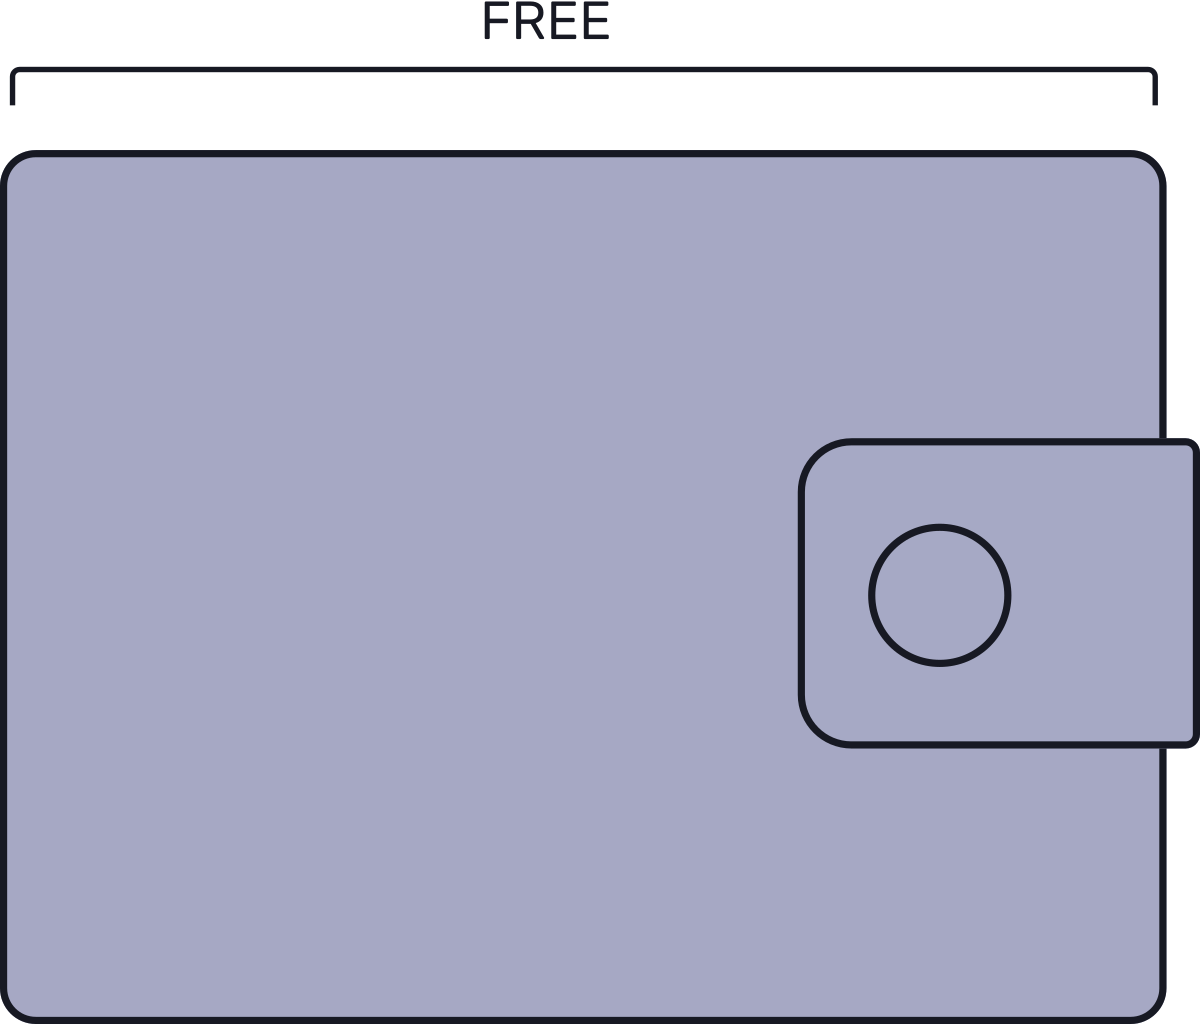
\includegraphics[width=0.60\textwidth]{img/wallet}
%    \end{subfigure}%
%    \begin{subfigure}{.5\textwidth}
%        \centering
%        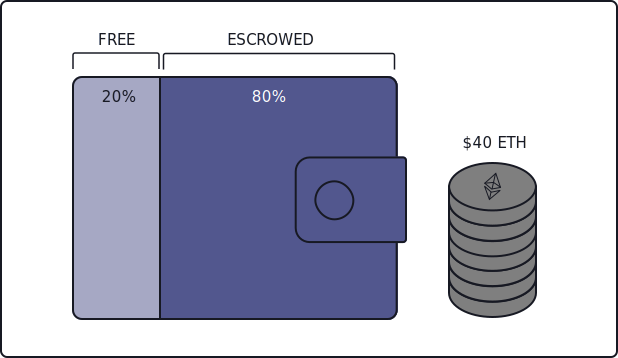
\includegraphics[width=0.80\textwidth]{img/escrowed}
%    \end{subfigure}
%\end{figure}

\begin{figure}[h!]
    \centering
    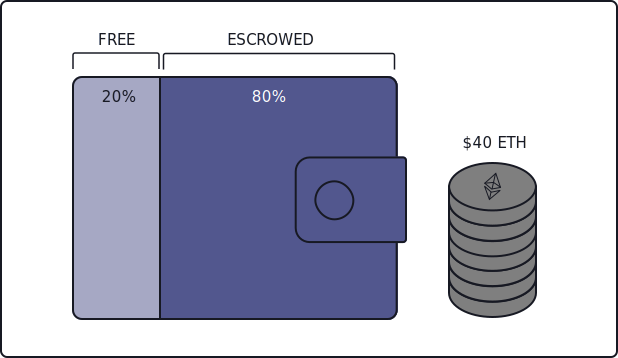
\includegraphics[width=0.40\textwidth]{img/escrowed}
\end{figure}

\vspace{2mm}

\noindent We now proceed to examine the respective consequences for Bob of nomin and havven
price shocks.

\newpage
\noindent \textbf{Nomin Price Shock} \\

\noindent This example shows how the system incentivises havven holders
to correct instability in the nomin price.

\begin{enumerate}
    \item{As a consequence of reduced demand in decentralised trading markets,
          the nomin price \(P_n\) drops to \$0.90. The system needs to incentivise havven
          holders to reduce the supply of nomins so that the price returns to \$1.00.
    }
    \item{First, consider that both \(C\) and \(C_{bob}\) have decreased to 0.36.
          Since the nomin price has changed, \(C_{opt}\) is recalculated to 0.342, which
          is smaller than both \(C_{bob}\) and \(C\). Consequently, \(C_{max}\) also changes
          to 0.4275. This increases the percentage of Bob's havvens that are locked.
    }

    \begin{figure}[h!]
        \centering
        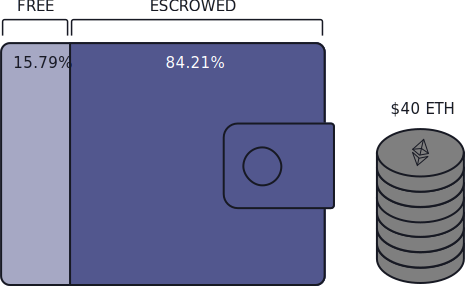
\includegraphics[width=0.4\textwidth]{img/pn_drop}
    \end{figure}

    \item{Bob now has a higher dollar value of locked havvens and \(C_{bob} > C_{opt}\).
          This means that he is no longer receiving the maximum fee rate
          \(\phi_{base}\). In order to return to \(\phi_{base}\) he must lower
          \(C_{bob}\) back to \(C_{opt}\) by burning some nomins. He needs to work out how
          many to burn.
    }

    \item{He should burn 2 nomins so that he has 38 total issued, which will cost
          \$1.80. When the system completes this process, his locked havvens will
          reduce back to 80. In addition, \(C_{bob}\) is equal to \(C_{opt}\) at 0.342,
          which means he is once again receiving the maximum fee rate.
    }
    \begin{figure}[h!]
    \centering
        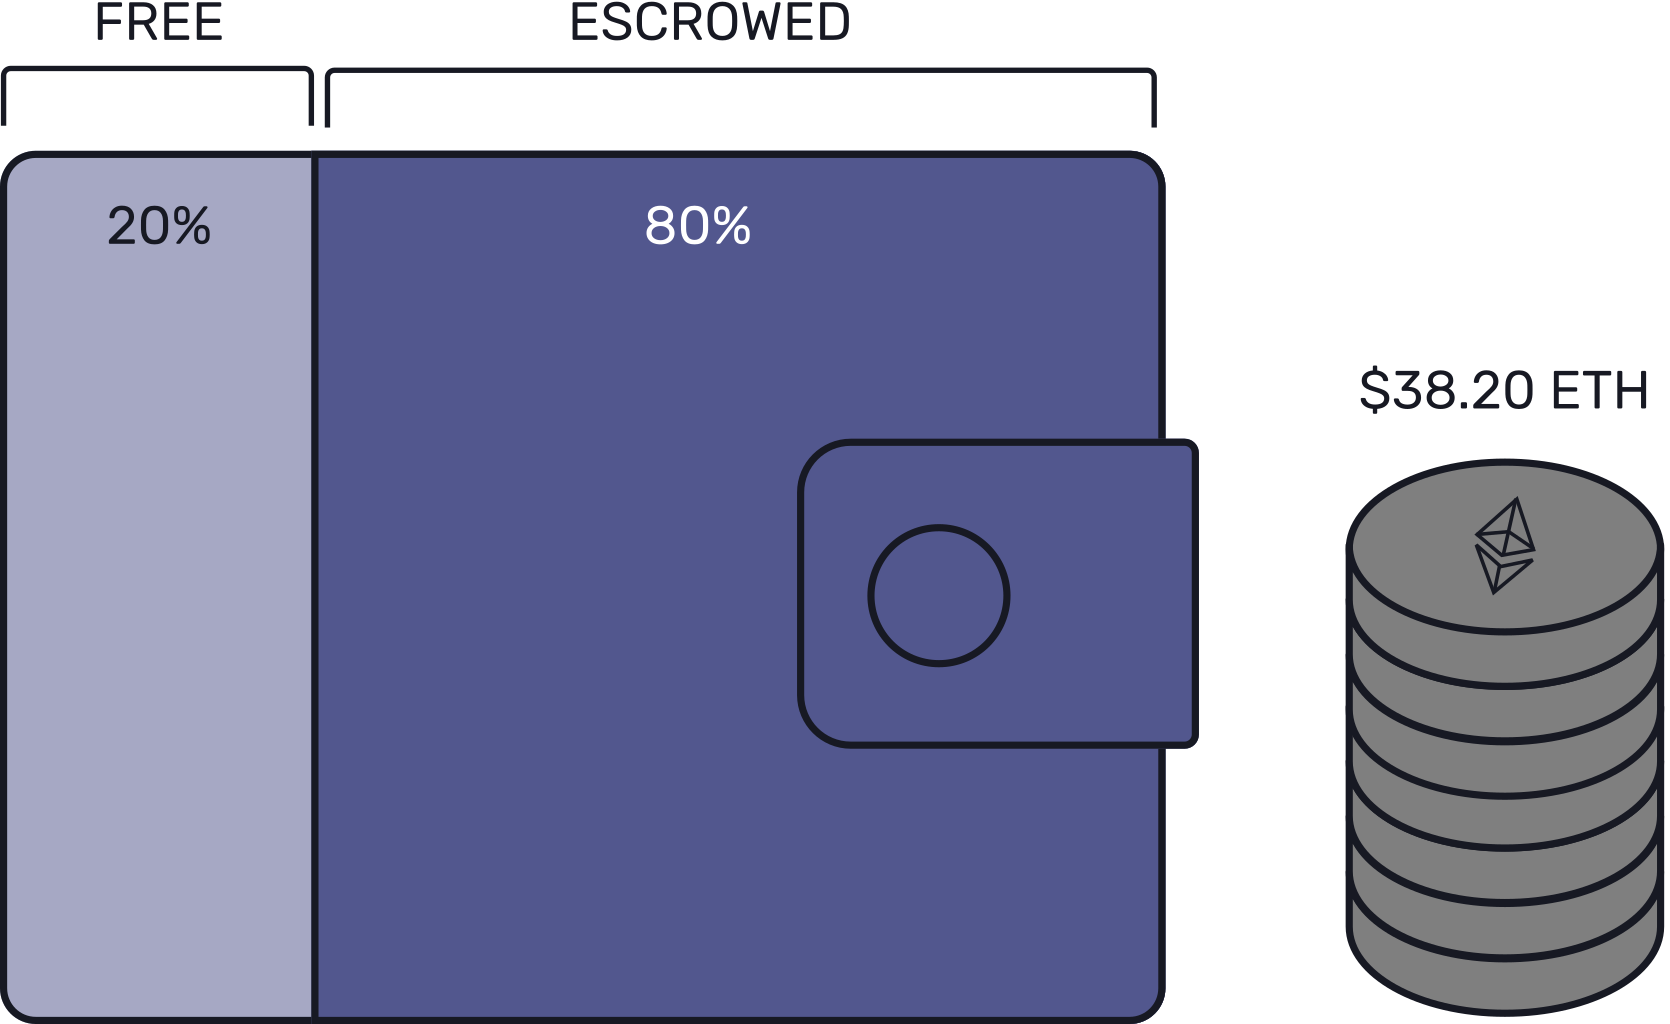
\includegraphics[width=0.4\textwidth]{img/post_burn}
    \end{figure}

    \item{Bob has taken the correct actions to raise the low nomin price. By
          electing to burn nomins, the system performed a limit buy order on his
          behalf, putting upward pressure on the nomin price. As compensation for doing
          so, he is rewarded with the optimal fee rate \(\phi_{base}\).
    }
\end{enumerate}


\newpage
\noindent \textbf{Havven Price Shock (Market Price)} \\

\noindent This example illustrates how the system maintains the dollar value of the underlying
collateral by adjusting the quantity of a user's escrowed havvens when the
havven price changes. We will use the same initial conditions as in the previous example.

\begin{enumerate}
    \item{As before, Bob elects to issue up to \(C_{opt}\) in order to maximise fees.}
    \begin{figure}[h!]
        \centering
        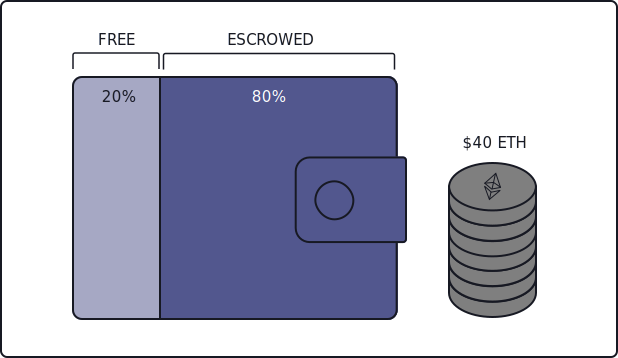
\includegraphics[width=0.4\textwidth]{img/escrowed}
    \end{figure}

    \item{The havven price \(P_h\) drops to \$0.90, which means the value of
          Bob's wallet has decreased to \$90. Both \(C\) and \(C_{bob}\) have increased to
          0.44. Since the nomin price has not changed, the system does not need to
          incentivise issuance or burning. This is reflected in the new value of
          \(C_{opt}\), which changes to 0.44, matching \(C\) and \(C_{bob}\).
    }

    \item{However, the system needs to escrow more of Bob's havvens to
          maintain the dollar value of the locked collateral. The system has now
          locked around 89\% of Bob's havvens, to maintain \$80 of locked
          collateral.
    }

    \begin{figure}[h!]
        \centering
        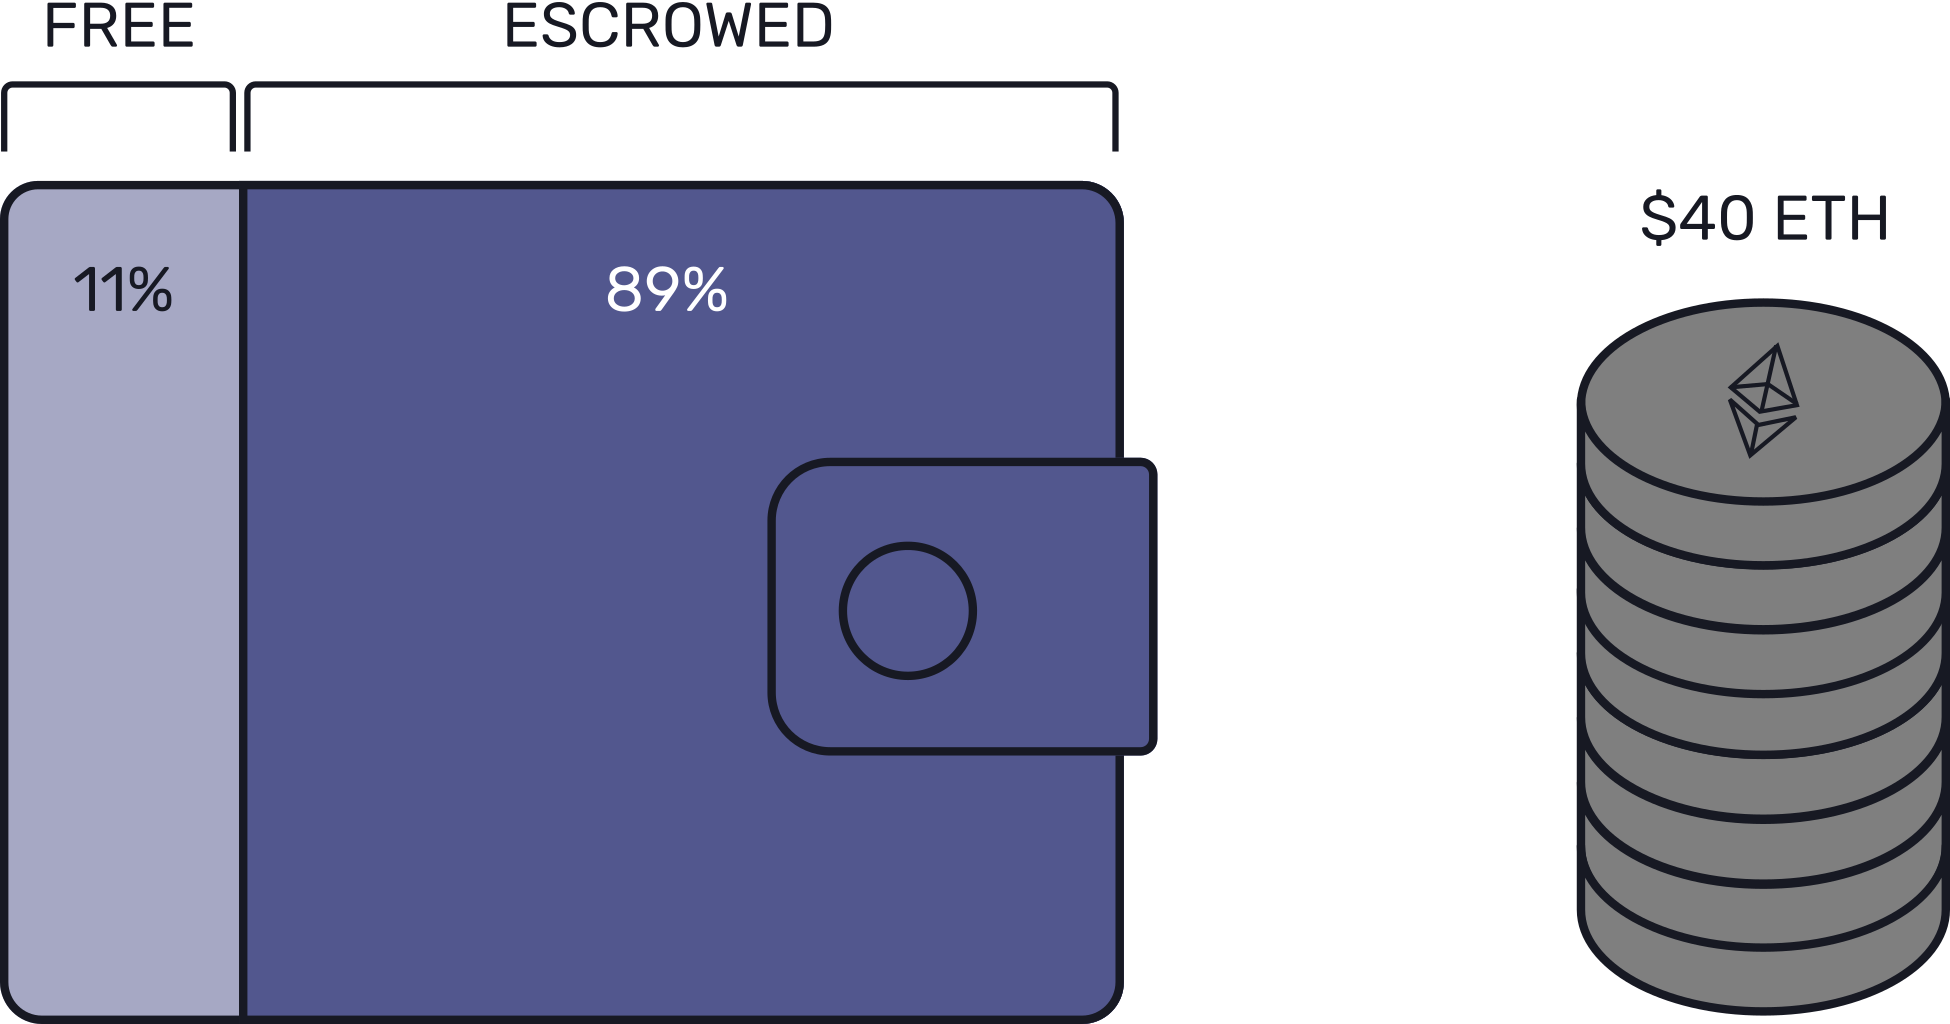
\includegraphics[width=0.5\textwidth]{img/ph_drop}
    \end{figure}
\end{enumerate} 


\newpage
\subsubsection{Optimality of Targeting \(C_{opt}\)}
\label{subsubsec:coptimality}

\noindent We will now examine the correct action for players to respond to changes in the
nomin price. The game begins in an equilibrium condition, with all players holding issuance
levels matching the optimal level. \\

\noindent For simplicity, we consider a system which has only two havven holders. We lose no generality
here, as a collection of actors behaving together can be considered as one agent. The sets of agents 
we consider are those those havven holders who do and do not respond to nomin price shocks by
matching their aggregated \(C_i\) to  \(C_{opt}\) as it changes, which is motivated by the
monotonicity of the fee function \eqref{eq:feesreceived} on either side of its maximum.

\noindent One player is assumed to own fewer havvens than the other. If this is not the case,
then in reality it soon will be if one strategy player's strategy is more profitable
than the other's. \\

\noindent We will examine each of the four cases describing how each player can act, and 
show that the correct action is for each player to target \(C_{opt}\). \\

\noindent \textbf{Initial Conditions and Definitions} \\

\noindent We denote the fraction of e-commerce transactions using nomins with \(\varepsilon \cdot GDP\) and
assume the following inverse demand function for the nomin price:

\begin{equation*}
    \label{eq:nominprice} P_{n,t} = \frac{\varepsilon \cdot GDP_t}{v_t \cdot N_t}
\end{equation*}

\vspace{2mm}

\noindent The expected profit of a havven holder \(i\) at period \(t\), with
respect to fees and their issuance actions can be expressed as follows:

\begin{equation*} 
    \pi_{i,t} = \phi_{r,i,t} \cdot \frac{H_{i,t}}{r} \ + \ (N_{i,t} - N_{i,t-1}) \cdot P_{n,t} \label{eq:profit}
\end{equation*}

\vspace{2mm}

\noindent The first havven holder owns 100 havvens and has
issued 50 nomins. The second owns 200 havvens and has issued 100 nomins.
Neither havven holder buys or sells havvens:

\begin{align*}
H &= 300 & H_1 &= 100 & H_2 &= 200 \\
N_{-1} &= 150 & N_{1,-1} &= 50 & N_{2,-1} &= 100
\end{align*}

\vspace{4mm}

\noindent The transaction fee rate (\(\phi_c\)), interest rate (\(r\)) and
velocity (\(v\)) are fixed throughout:

\begin{align*}
\phi_c &= 0.2\% & r &= 0.6\%  & v &= 6
\end{align*}

\vspace{4mm}

\noindent The values of the price sensitivity parameter (\(\sigma\)), the
flattening parameter (\(\psi\)) and the \(C_{max}\) multiplier (\(a\)) are:

\begin{align*}
\sigma &= 50 & \psi &= 3 & a&= 1.25
\end{align*}

\vspace{4mm}

\noindent To evaluate \(P_{n,-1}\) we assume that \(\varepsilon \cdot GDP_{-1} = 900\).
We can now also evaluate \(P_{h,-1}\) and the initial issuance ratios:

\vspace{2mm}

\begin{table}[!htbp]
    \centering
    \begin{tabular}{|m{1.2cm}|m{1.2cm}|m{1.2cm}|m{1.2cm}|m{1.2cm}|m{1.2cm}|m{1.2cm}|m{1.2cm}|}
        \hline
        \text{\(P_{n,-1}\)}&\text{\(P_{h,-1}\)}&\text{\(C_{-1}\)}&\text{\(C_{1,-1}\)}&\text{\(C_{2,-1}\)}&\text{\(f(P_{n,-1})\)}&\text{\(C_{opt,-1}\)}&\text{\(C_{max,-1}\)} \\
        \hline
        1 & 1 & 0.5 & 0.5 & 0.5 & 1 & 0.5 & 0.625 \\
        \hline
    \end{tabular}
    \caption{Prices and collateralisation; \(t = -1\)}
    \label{table:initial conditions}
\end{table}

\vspace{2mm}

\noindent The number of escrowed havvens for each havven holder is given by
equation \eqref{eq:escrowed}. We can also evaluate their expected profits:

\begin{align*}
    \check{H}_{1,-1} &= 80 & \pi_{1,-1} &= 100 \\
    \check{H}_{2,-1} &= 160 & \pi_{2,-1} &= 200 
\end{align*}

\vspace{4mm}

\noindent At the beginning of period \(t=0\), there is a 10\% decrease in
\(\varepsilon \cdot GDP\) causing the nomin price \(P_n\) to decrease from \$1 to
\$0.90, but neither player has yet reacted to the situation:

\begin{table}[!htbp]
    \centering
    \begin{tabular}{|m{1cm}|m{1cm}|m{1cm}|m{1cm}|m{1cm}|m{1cm}|m{1cm}|m{1cm}|}
        \hline
        \text{\(P_{n,0}\)}&\text{\(P_{h,0}\)}&\text{\(C_0\)}&\text{\(C_{1,0}\)}&\text{\(C_{2,0}\)}&\text{\(f(P_{n,0})\)}&\text{\(C_{opt,0}\)}&\text{\(C_{max,0}\)}\\
        \hline
        0.9 & 0.9 & 0.5 & 0.5 & 0.5 & 0.905 &  0.4525 & 0.5656 \\
        \hline
    \end{tabular}
    \caption{Negative shock; no reaction; \(t = 0\)}
    \label{table:Prices and collateralisation; t=0}
\end{table}

\vspace{2mm}

\noindent We now consider all possible combinations of actions in turn.
Either one, neither, or each player will react to bring their own issuance levels
into line with \(C_{opt}\). We examine the resulting expected profit for
each player in each situation and show that the correct action for both players
is to do so.

\newpage
\noindent \textbf{Neither Havven Holder Reacts} \\

\noindent If neither havven holder changes \(N_i\) then \(P_n\) will remain at \$0.90.
Altough for both havven holders \(\phi_{r,i,1} < \phi_{base,1}\), their
expected profits remain the same. This is because they have the same fee
rate, all fees must be distributed and collectively they own all havvens.
However, their number of locked havvens has increased:

\begin{align*}
    N_{1,1} &= 50 & \check{H}_{1,1} &= 88.4 & \pi_{1,1} &= 100 \\
    N_{2,1} &= 100 & \check{H}_{2,1} &= 176.8 & \pi_{2,1} &= 200 
\end{align*}

\vspace{4mm}

\noindent \textbf{Both Havven Holders React} \\

\noindent Instead of remaining idle, each havven holder has an opportunity to increase
\(\phi_{r,i,1}\) by changing \(N_{i,1}\) to align with \(C_{opt,0}\):

\begin{equation*}
    N_{i,1} = \frac{C_{opt,0} \cdot P_{h,0} \cdot H_i}{P_{n,0}}
\end{equation*}

\noindent If both havven holders target \(C_{opt}\), their new nomin balances,
locked havvens and expected profits are:

\begin{align*}
    N_{1,1} &= 45.25 & \check{H}_{1,1} &= 80 & \pi_{1,1} &= 86.22 \\
    N_{2,1} &= 90.5 & \check{H}_{2,1} &= 160 & \pi_{2,1} &= 172.45 
\end{align*}

\vspace{4mm}

\noindent Due to their actions, the nomin price, \(P_{n,1} \approx 1\),
\(f(P_{n,1}) \approx 1\) and \(C_{opt,1} \approx C_1\). There is no further
incentive for either havven holder to change \(N_i\). They also have reduced
\(\check{H}_i\) to the level it was originally:

\begin{table}[!htbp]
    \centering
    \begin{tabular}{|m{1cm}|m{1cm}|m{1cm}|m{1cm}|m{1cm}|m{1.5cm}|m{1cm}|m{1cm}|}
        \hline
        \text{\(P_{n,1}\)}&\text{\(P_{h,1}\)}&\text{\(C_1\)}&\text{\(C_{1,1}\)}&\text{\(C_{2,1}\)}&\text{\(f(P_{n,1})\)}&\text{\(C_{opt,1}\)}&\text{\(C_{max,1}\)} \\
        \hline
        0.9945 & 0.9 & 0.500 & 0.500 & 0.500 & 0.999 & 0.499  & 0.625 \\
        \hline
    \end{tabular}
    \caption{Negative shock; both react; \(t = 1\)}
    \label{table:negative shock both follow mechanism}
\end{table}

\vspace{2mm}

\noindent \textbf{Havven Holder 1 Reacts} \\

\noindent We now consider the scenario in which only the first havven holder changes
\(N_1\). We show the payoffs for each havven holder after 6 iterations. Havven
holder \(1\) improves his profit at the expense of havven holder \(2\):

\begin{align*}\label{pi_neg_shock_only N1_ t=6}
    N_{1,6} &= 46.57 & \check{H}_{1,6} &= 80 & \pi_{1,6} &= 118.53 \\
    N_{2,6} &= 100 & \check{H}_{2,6} &= 171.77 & \pi_{2,6} &= 171.58
\end{align*}

\noindent \(P_{n}\) stabilises around \(\$0.92\) instead of \(\$1\). The reason
being that, although \(P_n\neq 1\), \(C_{1,6} = C_{opt,6}\). This means that
havven holder \(1\) has no further incentive to change \(N_1\):

\begin{table}[!htbp]
    \centering
    \begin{tabular}{|m{1cm}|m{1cm}|m{1cm}|m{1cm}|m{1cm}|m{1.5cm}|m{1cm}|m{1cm}|}
        \hline
        \text{\(P_{n,6}\)}&\text{\(P_{h,6}\)}&\text{\(C_6\)}&\text{\(C_{1,6}\)}&\text{\(C_{2,6}\)}&\text{\(f(P_{n,6})\)}&\text{\(C_{opt,6}\)}&\text{\(C_{max,6}\)}\\
        \hline
        0.921 & 0.9 & 0.500 & 0.477 & 0.512 & 0.953 & 0.477  & 0.596 \\
        \hline
    \end{tabular}
    \caption{Negative shock; havven holder 1 reacts; \(t = 6\)}
\end{table}

\vspace{2mm}

\noindent \textbf{Havven Holder 2 Reacts} \\

\noindent Finally, we consider the case in which only havven holder \(2\) changes \(N_2\):

\begin{align*}
    N_{1,6} &= 50 & \check{H}_{1,6} &= 85.31 & \pi_{1,6} &= 77.25 \\
    N_{2,6} &= 93.78 & \check{H}_{2,6} &= 160 & \pi_{2,6} &= 204.90
\end{align*}
\vspace{4mm}

\noindent In this case, havven holder \(2\) improves his profit at the expense of
havven holder \(1\). Again, \(P_n\) does not stabilise at \(\$1\) but does
stabilise closer to \(\$1\) than in the previous scenario, since havven holder
\(2\) has a larger fraction of \(N\):

\begin{table}[!htbp]
    \centering
    \begin{tabular}{|m{1cm}|m{1cm}|m{1cm}|m{1cm}|m{1cm}|m{1cm}|m{1cm}|m{1cm}|m{1.5cm}|m{1cm}|m{1cm}|}
        \hline
        \text{\(P_{n,6}\)}&\text{\(P_{h,6}\)}&\text{\(C_6\)}&\text{\(C_{1,6}\)}&\text{\(C_{2,6}\)}&\text{\(f(P_{n,6})\)}&\text{\(C_{opt,6}\)}&\text{\(C_{max,6}\)}\\
        \hline
        0.939 & 0.9 & 0.500 & 0.522 & 0.489 & 0.978 & 0.489  & 0.612 \\
        \hline
    \end{tabular}
    \caption{Negative shock; havven holder 2 reacts; \(t = 6\)}
\end{table}

\vspace{2mm}

\noindent \textbf{Nash Equilibrium} \\

\noindent Both havven holders are best off by changing \(N_i\) to align with \(C_{opt}\).
Although for each of them the best scenario would be if the other does not do
anything, this scenario cannot be an equilibrium. This can be seen from the
following strategic game representation of the previous analysis (for this
representation, we assume that all iterations are made instantaneously and
simultaneously by both havven holders).

\begin{table}[!htbp]
    \centering
    \begin{tabular}{|c|c|c|}
        \hline
        \text{}&\text{\(N_{2,0}\)}&\text{\(N_{2}^*\)}\\
        \hline
        \text{\(N_{1,0}\)} & (100, 200) & (77.25, 204.9) \\
        \hline
        \text{\(N_{1}^*\)} & (118.53, 171.58) & (86.21, 172.43) \\
        \hline
    \end{tabular}
    \caption{Negative shock; strategic game representation}
    \label{table:negative shock_strateg game represent}
\end{table}
\vspace{2mm}

\noindent \(N_{i,0}\) is the action of maintaining the same number of nomins
taken by holder \(i\), whereas \(N_i^*\) is the action of changing their nomin
issuance. Each box has the payoff that both holders get by choosing some
particular action. For example, if havven holder \(1\) chooses \(N_{1,0}\) and
holder \(2\) chooses \(N_{2,0}\), the former gets a payoff of \(100\) and the
latter \(200\). It can be seen that havven holder \(1\) will choose \(N_{1}^*\) no
matter what action is chosen by havven holder \(2\) (\(1\) gets larger payoffs
following \(N_{1}^*\) for any action that \(2\) can take). Similarly, \(2\) will
choose \(N_{2}^*\) no matter what the action of havven holder \(1\) is. In other
words, action \(N_i^*\) strictly dominates remaining idle with \(N_{i,0}\).
Therefore, \(\{N_1^*,N_2^*\}\) is the unique Nash equilibrium. \\


\noindent \textbf{Other Conditions} \\

\noindent Note that the expected profit for each player decreases in the case of a negative price
adjustment. This is due to the fact that the players must buy back nomins from the market.
Yet this analysis does not take into account the profit obtained by later selling those nomins
in the case of a positive price adjustment. \\

\noindent The analysis for an isolated positive correction is similar to that for a negative one,
but since nomins are being issued rather than burnt, the nash equilibrium profits strictly increase
versus the "do nothing" scenario.
A table similar to the one above can be constructed for the case of a positive price shock:

\begin{table}[!htbp]
    \centering
    \begin{tabular}{|c|c|c|}
        \hline
        \text{}&\text{\(N_{2,0}\)}&\text{\(N_{2}^*\)}\\
        \hline
        \text{\(N_{1,0}\)} & (100, 200) & (100, 218.5) \\
        \hline
        \text{\(N_{1}^*\)} & (110.2, 200) & (114.7, 229.5) \\
        \hline
    \end{tabular}
    \caption{Positive shock; strategic game representation}
    \label{table:positive shock_strateg game represent}
\end{table}
\vspace{2mm}

\noindent In both cases the expected profit is positive; note that a balanced sequence of
positive and negative price shocks yields a positive expected profit. Thus in a steady
state havven holders should be able to profitably stabilise the system, and absorb modest
decreases in aggregate nomin demand.


\newpage


% \appendix
% \appendixpage
% \addappheadtotoc
%\section{Alternative approaches}

\todo[inline]{Establish a summary of arguments against each competitor}
\todo[inline]{Makerdao critique.}
\subsection{Basecoin}

\paragraph{Description of system}

\noindent Basecoin is described as operating similarly to Havven in that there is separation between a backing token and a transactional token, however Basecoin also separates out a specific ``bond'' token.
The peg to an arbitrary external asset is maintained by using an oracle service to discover the price on an external market, before regulating the supply of ``basecoins'' through actively increasing (issuing new basecoin),
and decreasing (auctioning of bonds) the supply, effectively acting as an autonomous central bank.

\subsubsection{Key issues}

\noindent Basecoin is intended to operate ``as a decentralized, protocol-enforced algorithm, without the need for direct human judgment (sic). For this reason,
Basecoin can be understood as implementing an algorithmic central bank.'' Whilst not without merit, this approach was discarded by Havven due to the high degree
of design complexity required to be anticipated in order to ensure the stabilisation mechanism is effective. The paper states that Monte Carlo simulations have
been run which indicate stability under a range of scenarios, however details are yet to be released by the team. \\

\noindent Another element not explored in the Basecoin whitepaper is the incentives for participants to engage with the cryptoeconomic system itself.
While there is no argument against the utility of stablecoins, there must be incentives inherent in all such systems to ensure the appropriate
participation of all actors. In this case, there are consumers of the stablecoin and active participants in the monetary policy. It is critical
to be able to demonstrate that the incentives within the system will ensure profitable participation strategies for actors. Without this being clarified
it is unclear as to whether there will be uptake by enough users to generate sufficient currency in circulation to support the demand for a stablecoin.
Critically, the removal of Basecoin from the system to ensure the stable peg is predicated on the significant assumption that participants will take positions
in the ongoing bond auctions. This assumption remains untested. \\

\noindent A final point needs to be made with respect to the overarching monetary approach
espoused in the whitepaper. In the section ``Averting Macroeconomic Depressions'' the authors appear to support
money printing and inflationary policies and the subsequent devaluation of currency. Even were it possible to
demonstrate that inflation of the money supply via such a system would be effective in combating a deflationary spiral,
a far better argument could be made that simply by implementing a stable store of value and unit of account that such a
system would not be required. Generally, the apparent assumption that such a system would be achievable and still able to
handle monetary crises in a far future time without centralised intervention stretches credulity. It's not entirely clear
why Basecoin has intended to merely replicate the function of a central bank, rather than aim for pure stability or a
relative-stable approach such as Havven. We are skeptical of any group that would advocate for monetary approaches that are
diametrically opposed to cryptoeconomic efforts to democratise money, and we feel that the proposal to intentionally
create a systematically inflationary monetary system is not the answer. Instead, we should at this point in time be
aiming to construct a system that provides a stable store of value relative to an arbitrary fiat currency. The macroeconomic
benefits of such a system are clear, and for as long as we live in a fiat-dominated world this will continue to be the case.

\subsection{Tether}

\paragraph{Description of system}

Tethers accepts fiat deposits into the Hong Kong-based Tether Limited bank account and issues ``USDT'' (USD Tether) over Bitcoin via the Omni Layer protocol. Tethers are an asset-backed digital token, representing a claim on the cash held in reserve. \\

\noindent The stability of the USDT `coin' effectively relies on the force of external market arbitrage to ensure the peg holds over time.

\paragraph{Key issues}

Despite the whitepaper claiming that the ``goal of any successful cryptocurrency is to completely eliminate the requirement for trust,'' and that each Tether is ``fully redeemable/exchangeable any time for the underlying fiat currency,'' the company's terms of service quite clearly state that ``there is no contractual right or other right or legal claim against us to redeem or exchange your Tethers for money.'' \\

\noindent Tether clearly relies on a manual, centralised proof of existence for the backing asset, and so suffers from the very issue that the Tether whitepaper decries. Indeed the same issue is encountered with tokenised gold, or similarly any other real-world asset where some Oracle bridge is required to interface into a distributed ledger.

\paragraph{Current state}

Recently, Tether announced support for issuing ERC-20 compatible tokens on Ethereum as opposed to releasing ``tethers'' on the Bitcoin blockchain using the Omni Layer protocol. \\

\noindent At the time of writing, the market capitalisation for USDT was approximately \$440m, and the discrepancy regarding their terms of service remains unresolved. \\


% \subsection{MakerDAO}

% \paragraph{Description of system}

% \paragraph{Key issues}

% \paragraph{Current state}

% \subsection{Nubits}

% \paragraph{Description of system}

% \paragraph{Key issues}

% \paragraph{Current state}

\pagebreak
%
\section{System variables}

%\todo[inline]{More complete system variable section.}

\noindent What follows are the main variables of the system. Under each heading, each row will correspond to a single quantity of interest. Each row will have three columns. Leftmost, a mathematical definition of the variable; in the middle, the dimension of the quantity (which units it is measured in); and on the rightmost, a short English summary of the variable.\\

\noindent Certain abbreviations will be used. For example, \(\HAV{}\) and \(\NOM{}\) will be used as abbreviations for havvens and nomins considered as units of measurement. \\

\paragraph{Prices}
\begin{align*}
    P_v & \ && &(\frac{\text{\$}}{\HAV{}}) && &\text{: havven price.} \\
    P_n & \ && &(\frac{\text{\$}}{\NOM{}}) && &\text{: nomin price.} \\
    \pi &:= \frac{P_v}{P_n} \ && &(\frac{\NOM{}}{\HAV{}}) && &\text{: havven to nomin conversion factor.} \\
    P_v' &= f(V_n, V_v) \cdot R && &(\frac{\text{\$}}{\NOM{} \cdot \text{sec}}) && &\text{: havven price rate of change.}
    \intertext{Here \(R\) is a risk term incorporating, for example, volatility, number of buyers versus sellers, and so on.}
\end{align*}
\\


\paragraph{Money Supply}
\begin{align*}
    &H \ && &(\HAV{}) && &\text{: Quantity of havvens, which is constant.} \\
    &H_e \ && &(\HAV{}) && &\text{: Quantity of escrowed havvens.} \\
    &N = H_N \cdot \pi \ && &(\NOM{}) && &\text{: Quantity of nomins. This can float.} \\
    &H_N = \frac{N}{\pi} \ && &(\HAV{}) && &\text{: Havven value of issued nomins.}
    \intertext{Ideally, \(H_N \leq H_e\).}
\end{align*}
\\

\paragraph{Utilisation Ratios}
\begin{align*}
    &U = \frac{H_N}{H} \ && &\text{(dimensionless)} && &\text{: Empirical issuance ratio. } \\
    &U_{max} \ && &\text{(dimensionless)} && &\text{: Targeted issuance ratio ceiling.}
    \intertext{\(0 \leq U \leq U_{max} \leq 1\)}
\end{align*}
\\

\paragraph{Microeconomic Variables} These should be defined as functions of \(P_n, \ P_v, \ \text{fees, etc.}\)
\begin{align*}
S_n \ && (\frac{1}{\text{sec}}) && &\text{: average nomin spend rate} \\
S_i \ && (\frac{1}{\text{sec}}) && &\text{: average issuance rate} \\
S_r \ && (\frac{1}{\text{sec}}) && &\text{: average redemption rate}
\end{align*}
\\

\paragraph{Money Movement}
\begin{align*}
    V_n &= S_n \cdot N \ && &(\frac{\NOM{}}{\text{sec}}) && &\text{: nomin transfer rate.} \\
    V_v &= V_i + V_r \ && &(\frac{\HAV{}}{\text{sec}}) && &\text{: nomin} \leftrightarrow \text{havven conversion rate.} \\
    V_i &= (H - H_N) \cdot S_i \ && &(\frac{\HAV{}}{\text{sec}}) && &\text{: nomin issuance rate.} \\
    V_r &= H_N \cdot S_r \ && &(\frac{\HAV{}}{\text{sec}}) && &\text{: havven redemption rate.} \\
    \intertext{\(V_i\) is assumed to grow as there are more free havvens in the system.}
    \intertext{\(V_r\), by contrast, is taken to grow proportionally with the number of escrowed Havvens.}
\end{align*}
\\

\paragraph{Fees}
\begin{align*}
\intertext{The following fees are ratios, for example 0.1\%, levied on each transaction.}
&F_{nx} & \ && &\text{(dimensionless)} && &\text{: nomin transfer fee} \\
&F_{vx} & \ && &\text{(dimensionless)} && &\text{: havven transfer fee} \\
&F_i & \ && &\text{(dimensionless)} && &\text{: nomin issuance fee} \\
&F_r & \ && &\text{(dimensionless)} && &\text{: havven redemption fee} \\
% \intertext{These quantities are the aggregated fees accrued by the system per unit time.}
% &Ag_{nx} &:= V_n \cdot F_{nx} \ && &(\frac{\NOM{}}{\text{sec}}) && &\text{: fees taken from nomin transfers.}
\end{align*}

\pagebreak


%\bibliography{tex/citations}
%\bibliographystyle{plain}

\end{document}
